\begin{titleDef}{Die Poincaré-Halbebene/Halbebenen-Modell}
\label{hyperbolischpoincare}
Die \textbf{Poincaré-Halbebene} oder \textbf{Halbebenen-Modell} ist ein Modell für hypergeometrische Geomtrie\\
Sie wird beschrieben durch die obere Halbebene $H^2=\{(x,y)\in\Rtwo|\ y>0\}$ versehen mit der \hyperref[riemannMetrik]{Riemannschen Metrik} $g_{ij}=\frac{\delta_{ij}}{y^2}$ d.h:
$$(g_{ij}(u_1,u_2))=\begin{pmatrix}
	\frac{1}{y^2}&0\\0&\frac{1}{y^2}
\end{pmatrix}
$$
Bildlich führt das so definierte Skalarprodukt dazu, dass das Skalarprodukt eines Vektors unendlich groß wird, je näher er an die x-Achse kommt also je kleiner die y-Komponente wird. Der Raum $\Rtwo$ wird also nach oben hin gestreckt und nach unten unendliche gestaucht.\par
Anstelle von reellen Koordinaten $(x,y)\in\Rtwo$ verwendet man in der regel alternativ komplexe Koordinaten $z=x+iy\in\mathbb{C}$ und somit\\ $H^2=\{z\in\mathbb{C}|\ Im(z)>0\}$
\end{titleDef}

\begin{titleDef}{hyperbolische Länge}
\label{hyperLaenge}
Für eine stückweise \hyperref[kurve]{differenzierbare} Kurve
$$c:[a,b]\to H^2;\: t\mapsto c(t)=(x(t),y(t))$$
definiert man die \textbf{hyperbolische Länge}
$$L_h(c)=\int_{a}^{b}\lVert c^\prime(t)\rVert_{c(t)} dt=\int_{a}^{b}\frac{\sqrt{(x^\prime(t))^2+(y^\prime(t))^2}}{y(t)}dt$$
In der komplexen Darstellung gilt für die Kurve: $c(t)=z(t)=x(t)+iy(t)$ und damit:
$$L_h(c)=\int_{a}^{b}\lVert z^\prime(t)\rVert_{z(t)}=\int_{a}^{b}\frac{\lvert z^\prime(t)\rvert}{Im(z(t))}$$
Beachte das wegen der konvergenz des Skalarprodukts gegen $\infty$ für $y\to 0$ folgt das $L_h(c)\to\infty$ für $a\to 0$.\par
Die hyperbolische Länge ist invariant unter \hyperref[moebiustrans]{Möbiustransformationen} von $H^2$. D.h für eine differenzierbare Kurve $c$ in $H^2$ gilt: $L_h(c)=L_h(T_A\circ c)$
\end{titleDef}

\begin{titleDef}{hyperbolischer Flächeninhalt}
\label{hyperFlaeche}
Für eine Teilmenge $G\subset H^2$ von $H^2$ ist der \textbf{hyperbolische Flächeninhalt} definiert durch:
$$0\leq\mu(G)=\int\int_{G}\frac{1}{y^2}dxdy\leq\infty$$
Der \textbf{hyperbolische Flächeninhalt} ist invariant unter \hyperref[moebiustrans]{Möbiustransformationen}.\\
d.h. Falls $G\subset H^2$ und $\mu(G)$ existiert so ist für alle $A\in SL(2,\mathbb{R}): \:\: \mu(G)=\mu(T_A(G))$ 
\end{titleDef}

\begin{titleDef}{Geodätische Linien der Poincaré-Ebene}
\label{geodaetischPoincare}
In der Poincaré-Halbebene gibt es zwei Formen von \hyperref[geodaetischeLinie]{\textbf{Geodätischen Linien}}. 
\begin{itemize}
	\item Einmal klassische Geraden die parallel zu der y-Achse laufen, da diese kürzeste Verbindungen von zwei Punkten beschreibt, die gleiche x-Komponente haben da die definierte Riemannsche Metrik nur von y-abhängt.
	\item Die zweite Art von Geodätischen sind Halbkreise, die die beiden Punkte auf ihrem Rand schneiden, die eine kürzeste Verbindung von zwei Punkten darstellt, die verschiedene x-Komponenten haben, selbst wenn die y-Komponente übereinstimmt da hier der invers, quadratische Faktor von y ins Spiel kommt
\end{itemize}
Formal gilt: Die kürzeste Verbindungskurven zwischen zwei Punkten in der hyperbolischen Ebene $H^2$ sind (mit hyperbolischer \hyperref[bogenlaenge]{Bogenlänge} parametrisierte) Halbkreise und Geraden orthogonal zur reellen Ebene bzw der x-Achse. Solche Kurven sind genau die \textbf{geodätischen Linie} in $H^2$.\\
Je zwei Punkte $p,q\in H^2$ können durch eine eindeutige geodätische Linie verbunden werden und der hyperbolische Abstand $d_h(p,q)$ entspricht gerade der Länge dieses geodätischen Segments. \\
Die Halbkreise die geodätische Linien sind haben ihren Mittelpunkt auf der reellen-/x-Achse.
\begin{figure}[h]
	\centering
	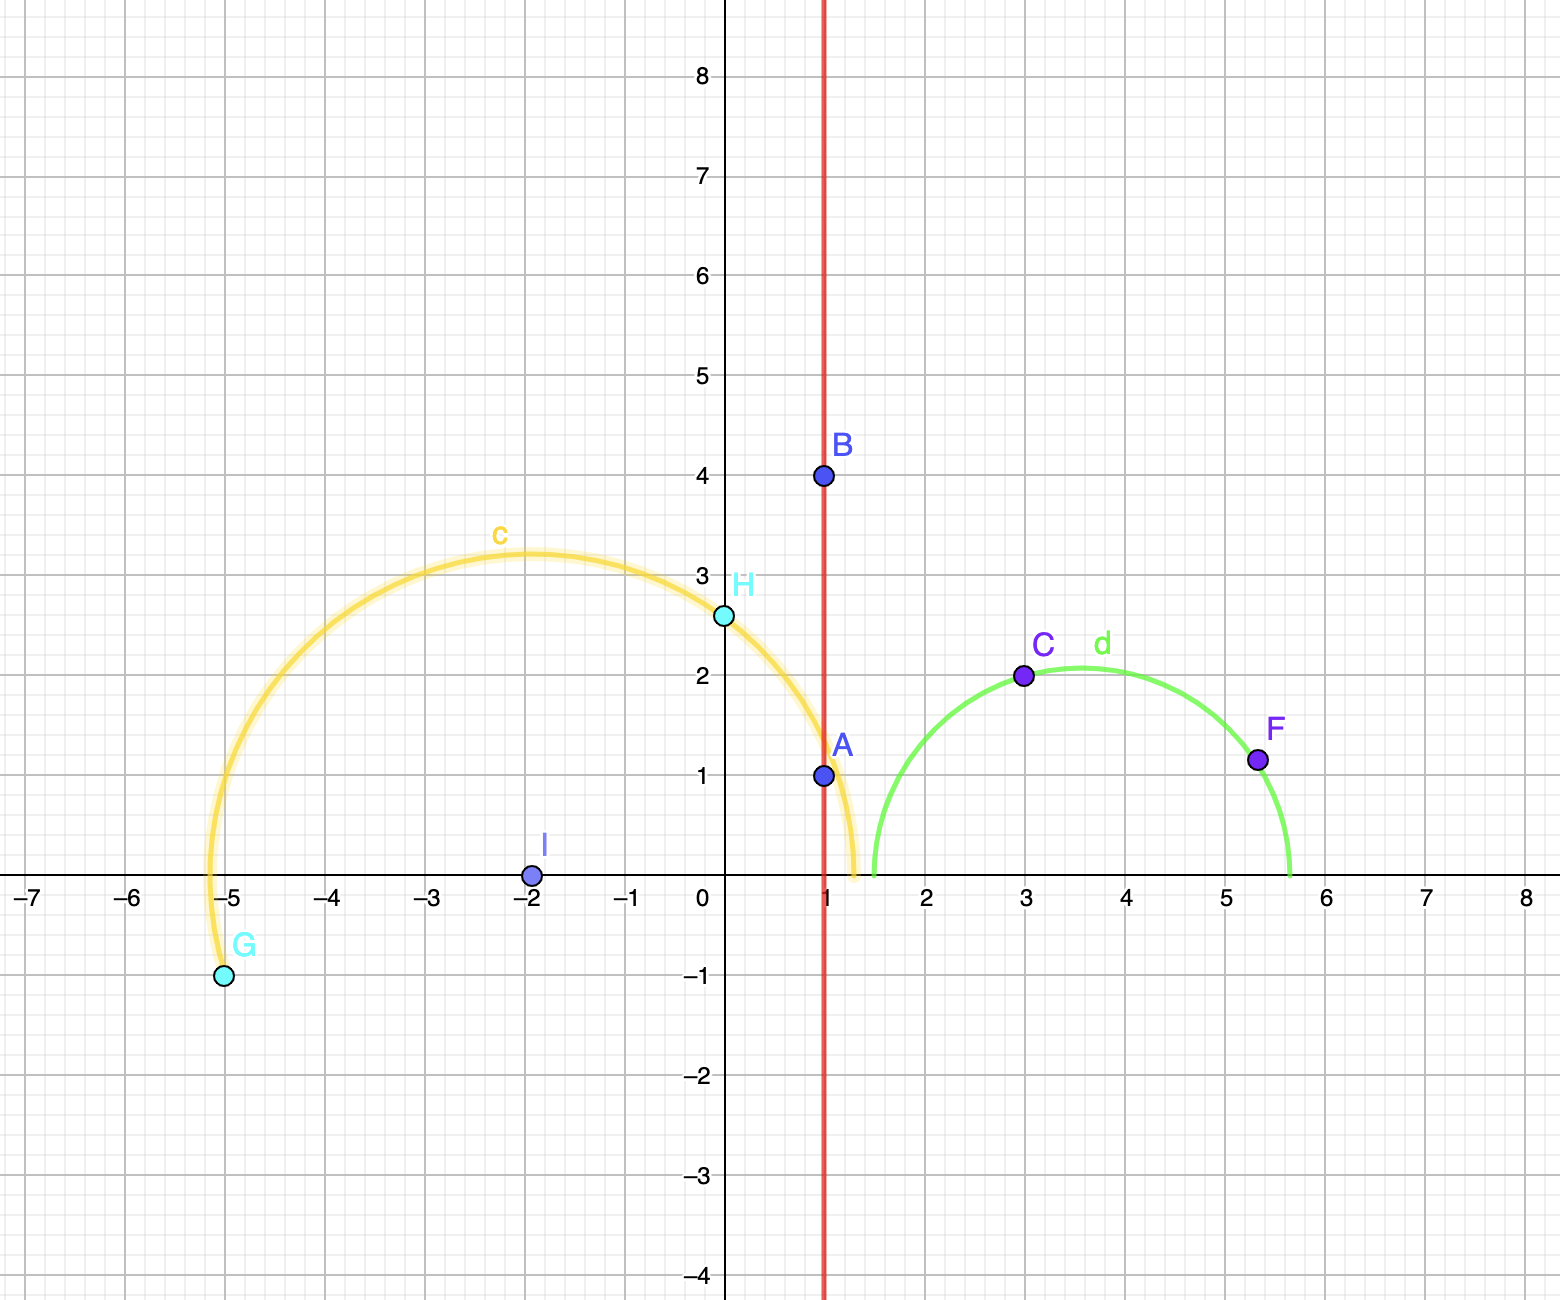
\includegraphics[width=\linewidth]{Bilder/GeodaetischeHyperebene}
	\label{geodaetischeHyperGrafik}
\end{figure}
\end{titleDef}

\begin{titleDef}{Beispiel Bogenlänge parametrisierte imaginäre Achse}
\label{parametrisierungImaginaer}
Hyperbolische geodätische Linien in $X=H^2$ sind genau die Bilder von \hyperref[abstandserhaltend]{abstandserhaltenden} Abbildungen $\gamma:\mathbb{R}\to X$ mit $d_h(\gamma(t_1),\gamma(t_2))$ für den (Bogenlängen-)parameter $t$.\\
Die Parametrisierung der imaginären-/y-Achse nach hyperbolischer \hyperref[bogenlaenge]{Bogenlänge} ist gegeben durch:
$$A_t=\begin{pmatrix}
	e^{\frac{t}{2}}&0\\0&e^{-\frac{t}{2}}
\end{pmatrix},\: \gamma(t)=T_{A_t}(i)=\frac{e^{\frac{t}{2}}i+0}{0i+e^{-\frac{t}{2}}}$$
Damit gilt für $t_2\geq t_1$:
$$d_h(\gamma(t_1),\gamma(t_2))=d_h(e^{t_1}i,e^{t_2}i)=\ln e^{t_2}-\ln e^{t_1}=t_2-t_1$$
damit ist $t$ Bogenlängenparameter.
\end{titleDef}

\newpage
\begin{titleDef}{Abstand von Punkten auf der imaginären Achse}
\label{abstandhyperIm}
Für den Abstand von zwei Punkten $t_1,t_2\in H^2$ die auf der imaginären Achse liegen, d.h
$t_1=\lambda_1i,t_2=\lambda_2i,\lambda_1,\lambda_2\in\mathbb{R}$ gilt:
$$d_h(t_1,t_2)=d_h(\lambda_1i,\lambda_2i)=\lvert ln(\lambda_2)-ln(\lambda_1)\rvert$$
Der einfachheithalber ändere o.B.d.A die Komponenten sodass man den größeren Wert vom kleineren subtrahiert.\\
$$d_h(2i,\frac{1}{2}i)=\lvert\ln(\frac{1}{2})-\ln(2)\rvert=\lvert\ln\left(\frac{\frac{1}{2}}{2}\right)\rvert=\lvert\ln(\frac{1}{4})\rvert=\lvert\ln(1)-\ln(4)\rvert=\lvert0-\ln(4)\rvert=\lvert -2\ln(2)\rvert=2\ln(2)$$
$$d_h(\frac{1}{2}i,2i)=\lvert\ln(2)-\ln(\frac{1}{2})\rvert=\lvert\ln(\frac{2}{\frac{1}{2}})\rvert=\lvert\ln(4)\rvert=\lvert2\ln(2)\rvert=2\ln(2)$$
\end{titleDef}

\begin{titleDef}{Möbiustransformation von geodätischen auf die y-Achse}
Sei $L$ ein euklidischer Halbkrei oder eine Halbgerade in $H^2$, welche die reelle-/x-Achse in einem Punkt $\alpha$ orthogonal schneidet, also ist $L$ gerade eine geodätische Linie in der hyperbolischen Ebene. \\
Dann ist $T(z)=-\frac{1}{z-\alpha}+\beta,\: \beta\in\mathbb{R}$ eine Möbiustransformation die $L$ für ein geeignetes $\beta$ auf die imaginäre-/y-Achse abbildet. d.h es existiert ein $A\in SL(2,\mathbb{R})$ so, dass $T=T_A$. Also gibt es eine Möbiustransformation die eine geodätische Linie auf die imaginäre-/y-Achse abbildet also insbesondere die Punkte die durch diese verbunden werden wobei die Länge zwischen diesen erhalten bleibt, da Möbiustransformationen Isometrien sind.
\end{titleDef}

\begin{titleDef}{Möbiustransformation}
\label{moebiustrans}
Für eine Matrix $$A\in SL(2,\mathbb{R}),\: A=\begin{pmatrix}
	a&b\\c&d
\end{pmatrix},\: det(A)=ad-bc=1$$
definiere die \textbf{Möbiustransformation}
$$T_A:H^2\to H^2;\: z\mapsto\frac{az+b}{cz+d}$$
Es gilt $(T_A)^{-1}=T_{A^{-1}}$\par
Die Möbiustransformation entspricht der Translation und Rotation von euklidischen Ebenen.
\par
Die Möbiustransformationen $\{T_A|\ A\in SL(2,\mathbb{R})\}$ sind \hyperref[Isometrie]{Isometrien} der hyperbolischen Ebene $(H^2,d_h)$ also insbesondere \hyperref[abstandserhaltend]{abstandserhaltend}.\par
Für beliebige Punkte $p,q\in H^2$ existiert eine Isometrie/Möbiustransformation $T_A$ so, dass $T_A(p)=q$.
\end{titleDef}

\begin{titleDef}{Streckung in Hpyerbolischer Ebene}
\label{hyperStreckung}
In der hyperbbolischen Ebene $H^2$ ist die Streckung der Fläche um $\lambda\in\mathbb{R}_{>0}$ ist gegeben durch $s_\lambda:H^2\to H^2$ und wird durch eine \hyperref[moebiustrans]{Möbiustransformation} definiert:
$$s_\lambda=T_A \: \text{für} \: A=\begin{pmatrix}
	\sqrt{\lambda}&0\\0&\frac{1}{\sqrt{\lambda}}
\end{pmatrix}$$
Insondere gibt es also beliebig viele verschiedene streckungen der hyperbolischen Ebene und jede ist eine \hyperref[Isometrie]{Isometrieå} anders als in der euklidischen wo die einzige Streckung die gleichzeitig eine Isometrie ist die Identität ist.
\end{titleDef}



\begin{titleDef}{Hyperbolische Ebene als Metrischer Raum}
\label{hyperToMetrisch}
Nachdem man nun auf der hyperbolischen Ebene $H^2$ mit dem Halbebenen-Modell eine Längenmetrik durch die \hyperref[hyperLaenge]{hypergeometrische Bogenlänge} definiert hat kann man diese nun zu einem \hyperref[MetrischerRaum]{Metrischen Raum} erweitern.\par
Definiere dazu für Punkte $p,q\in H^2$ die Menge $\Omega_{pq}$ als die Menge aller stückweise differenzierbaren \hyperref[kurve]{Kurven} zwischen $p$ und $q$. Dann wird durch
$$d_h(p,q)=\inf\{L_h(c)|\ c\in\Omega_{pq}\}$$
eine Metrik definiert und $(H^2,d_h)$ ist ein \hyperref[MetrischerRaum]{metrischer Raum}
\end{titleDef}

\begin{titleDef}{Unendlicher Rand}
\label{unendlicherRand}
Man kann die hyperbolische Ebene "kompaktifizieren" indem man die reelle-/x-Achse und einen Punkt $\infty$ hinzunimmt: $\overline{H^2}=H^2\cup(\mathbb{R}\cup\{\infty\})$.\\
Das ist zu verstehen als alle Punkte die von einem Punkt $i$ in jeder Richtung unendlich weit entfernt sind.\\
Die Menge $\partial_\infty H^2=\mathbb{R}\cup\infty$ heißt der \textbf{unendliche Rand} von $H^2$.
\end{titleDef}

\begin{titleDef}{hyperbolische Dreiecke}
\label{hyperDreieck}
Ein \textbf{hyperbolisches Dreieck} $\Delta\subset\overline{H^2}$ ist eine \hyperref[konvexPoly]{konvexe} Teilmenge (d.h für zwei Punkte $p,q\in\Delta$ liegt auch das Geradensegment $\overline{pq}$ ganz in $\Delta$) begrenzt von 3 Segmenten von \hyperref[geodaetischPoincare]{geodätischen Linien}, die sich paarweise in Punkten $A,B,C$ den \textbf{Ecken} des Dreiecks schneiden. Die Ecken $A,B,C$ dürfen dabei im \hyperref[unendlicherRand]{unendlichen Rand} $\partial_\infty H^2=\mathbb{R}\cup\{\infty\}$ liegen, die Seiten jedoch nicht.\par
\label{hyperInnenwinkel}
Der \textbf{Innenwinkel} $\varphi$ in einer Ecke $E$ eines Dreickes ist definiert durch die zugrundeliegende \hyperref[riemannMetrik]{Riemannsche Metrik} als die entsprechenden Winkel zwischen den \hyperref[tangentialvektor]{Tangentialvektoren} an die \hyperref[geodaetischPoincare]{geodätischen Linien} wie \hyperref[kennwerteRiemann]{hier} definiert, falls die Ecke in $H^2$ liegt. Falls die Ecke auf dem \hyperref[unendlicherRand]{unendlichen Rand} liegt setzte $\varphi=0$\\
Beachte das der hyperbolische Winkel mit dem euklidischen Winkel übereinstimmt obwohl die hyperbolische Länge sich anders verhält als die euklidische Länge.
\end{titleDef}

\begin{titleDef}{Gauß-Bonnet für hyperbolische Dreiecke}
\label{gaussHyperDreieck}
Der \hyperref[hyperFlaeche]{hyperbolische Flächeninhalt} eines \hyperref[hyperDreieck]{hyperbolischen Dreiecks} $\Delta$ ist durch die drei Innenwinkel $\alpha,\beta,\gamma$ bestimmt und durch $\pi$ beschränkt.
$$0\leq\mu(\Delta)=\pi-(\alpha+\beta+\gamma)$$
Insbesondere ist also $\alpha+\beta+\gamma<\pi$ und $\mu(\Delta)<\pi$
\end{titleDef}